\documentclass[a4paper,11pt]{article}
\usepackage[utf8]{inputenc}
\usepackage[T1]{fontenc}
\usepackage{amsmath}
\usepackage{mathtools}
\usepackage{amsfonts}
\usepackage{amssymb}
\usepackage{graphicx}
\usepackage{multicol}
\usepackage{array}
\usepackage{float}
\usepackage{epstopdf}
\usepackage{caption}
\usepackage{subcaption}
\usepackage{gensymb}
\usepackage[bottom]{footmisc}
\usepackage{appendix}
\usepackage{pdfpages}
\usepackage{todonotes}
\usepackage{mathpazo}
\usepackage{titleps}
\usepackage{color}
\usepackage{xcolor}
\usepackage{colortbl}
\usepackage{siunitx}
\usepackage{pdflscape}
\usepackage{cancel}

\usepackage[skins]{tcolorbox}
\usepackage{sectsty}
\usepackage[arrowmos]{circuitikz}
\usepackage{pgfplots}
\usepackage{blindtext}
\usepackage[inner=2cm,outer=2cm,top=2.5cm,bottom=2.5cm]{geometry}
\usepackage{todonotes}
\usepackage{hyperref}
\usepackage{url}
\usepackage{adjustbox}
\usepackage{tabularx}
\usepackage{booktabs}
\usepackage{fancybox}
\usepackage[tikz]{bclogo}


%For code insertion
\usepackage{listings}
\lstdefinestyle{customc}{
  belowcaptionskip=1\baselineskip,
  breaklines=true,
  frame=L,
  xleftmargin=\parindent,
  language=C,
  showstringspaces=false,
  basicstyle=\footnotesize\ttfamily,
  keywordstyle=\bfseries\color{green!40!black},
  commentstyle=\itshape\color{purple!40!black},
  identifierstyle=\color{blue},
  stringstyle=\color{orange},
}

\lstdefinestyle{customasm}{
  belowcaptionskip=1\baselineskip,
  frame=L,
  xleftmargin=\parindent,
  language=[x86masm]Assembler,
  basicstyle=\footnotesize\ttfamily,
  commentstyle=\itshape\color{purple!40!black},
}

\lstset{escapechar=@,style=customc}
%End for code insertion


\graphicspath{{figures/}}
\sectionfont{\large}
\subsectionfont{\normalsize}

%%%%%%%%%%%%%%%%%%%
% HANDS-ON NUMBER
\newcommand\handsOnN{}
% WEEK NUMBER
\newcommand\weekN{2}
%%%%%%%%%%%%%%%%%%%

\newpagestyle{main}{
	\sethead[LELEC2102: Hands-on \handsOnN][][]{LELEC2102: Hands-on \handsOnN}{}{}
	\headrule
    \setfoot[][\thepage][]{}{\thepage}{}
}

\newcommand{\horrule}[1]{\rule{\linewidth}{#1}} % Create horizontal rule command with 1 argument of height

%%%%%%%%%%%%%%%%%%%%%%%%%%%%%%%%%%%%%%%%%%%%%%%%%%%%%%%%%%%%%%%%%%%%%%%%%%%%

\begin{document}
\renewcommand{\figurename}{Fig.}

\renewcommand{\thepage}{\arabic{page}}
\setcounter{page}{1}
\pagestyle{main}
\newpage \clearpage

\begin{center}
\begin{huge}
Hands-On: MCU operation and baremetal programming\\
\end{huge}
\vspace{0.3cm}
%\textit{TA 1, TA 2}
\end{center}

\section*{Introduction}

GNU radio uses software to command various block, allowing to rapidly construct and test communication blocks. It can be interesting to be able to create your own blocks and to dynamically update parameters of a block from another one. For example, the LimeSDR parameters, such as the gain, can be modified from GNU radio. It is however not trivial and we will will decompose this into two steps. The first one is to dynamically update a GNU radio variable from a given block. The second one is to automatically get the updated value of this variable in another block. In this tutorial, you will therefore learn the following manipulations:

\begin{itemize}
    \item How to create a new block in GNU radio.
    \item How to update dynamically a GNU radio variable.
    \item How to get the updated value of a variable automatically.
\end{itemize}

Finally, we will quickly discuss some important points regarding the update of LimeSDR parameters from GNU Radio.

\section*{Objectives}

\begin{itemize}
    %\item Learn the basics of audio sampling in an embedded context ;
%    \item Learn how to add a new peripheral to a project ;
    \item Learn about new peripherals : ADC and DMA ;
    \item Learn how to set up these peripherals for audio acquisition ;

    %\item Learn how to use an ADC on a STM32 MCU and sample at a given frequency using a TIMER ;
    %\item Learn how to use a DMA to offload some workload on the MCU ;
    \item Learn how to implement a double buffering approach ;
    %\item Learn more about the AFE part of the custom board and understand how to configure it ;
    \item Learn how to acquire your audio data from the UART interface and generate an audio file.
\end{itemize}

\section*{Material \& preparation}

\begin{comment}[couleur = gray!20, arrondi = 0.2, logo=\bcinfo]{}
\vspace{0.2cm}
\end{comment}
For this hands-on session, you will need:
\begin{itemize}
    \item The Nucleo MCU board with its sensing and power-management board ;
    \item A USB cable to connect your computer to the Nucleo;
    \item A LimeSDR connect to the MCU with a SMA cable.
\end{itemize}

\section{Setting up the VM}
To program and debug an MCU, we use an Integrated Development Environbment (IDE). For the Nucleo MCU board, we use the STM32Cube IDE, which is preinstalled on the VM we provided you. You simply have to open it. However, when plugging in your Nucleo MCU board, it is connected to your host system. In the next steps, we will show you how to perform an USB passthrough such that the Nucleo MCU board will connect to your virtual machine. This step will need to be done everytime you plug in your board \footnote{Our explanations assume you have a Windows host OS, if your host OS is Linux, some additional steps have to be done. Please follow the separate tutorial on Moodle or at \url{https://www.linuxbabe.com/virtualbox/access-usb-from-virtualbox-guest-os}}.\\

Launch your VM. After the boot, you can plug in your Nucleo MCU board, it will show up in the host OS. Then, in Virtual Box, under Devices $\rightarrow$ USB, select \textbf{STMicroelectronics STM32 STLink} as in \autoref{fig:usb_passthrough}.
\begin{figure}[H]
    \centering
    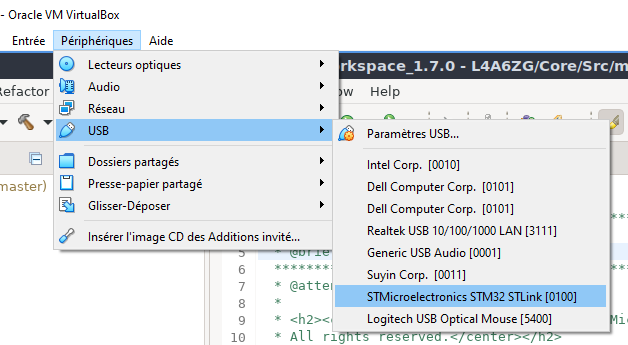
\includegraphics[scale=0.6]{figures/usb_passthrough.png}
    \caption{Nucleo VM configuration}
    \label{fig:usb_passthrough}
\end{figure}
Now, the Nucleo should be connected to your VM. \\
%
\textbf{If you do not see the toolbar}, go back to Virtual Box,
right click on your virtual OS, go to \emph{User Interface} and ensure the boxes are checked, as shown in Figure~\ref{fig:toolbar}. It can happen that you don't see it because of the \emph{Monitor settings}. In this case, press "\emph{Host Key}"+"\emph{F}" ("\emph{Host Key}" is "\emph{Right control}" in Windows 10) once or twice and the toolbar should appear. \\
If it still does not work, a last possibility is to press "\emph{Right Control}" + "\emph{Home}" on the virtual OS. It will pop up as a contextual menu through which you will be able to reactivate the display of the menu.

\begin{figure}[H]
    \centering
    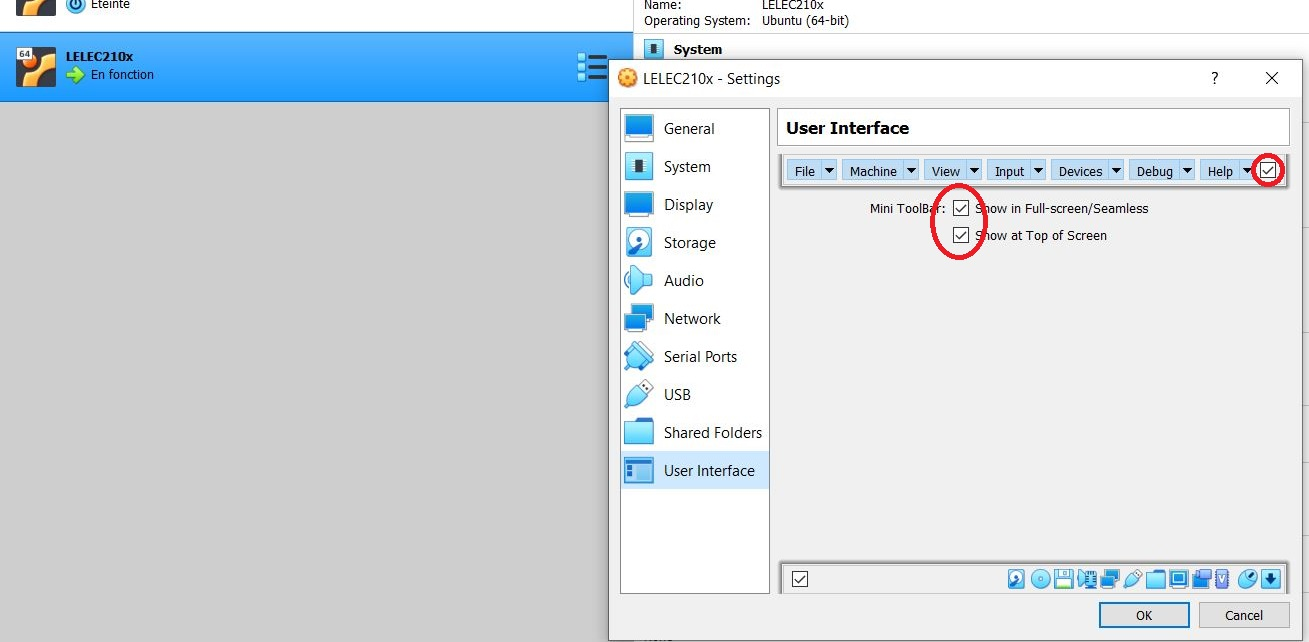
\includegraphics[width = 0.65\linewidth]{figures/toolbar.JPG}
    \caption{Viewing the toolbar.}
    \label{fig:toolbar}
\end{figure}
%
\section{Practical part}

\subsection{Starting from the baseline version}

As mentioned in the introduction, you will not start from scratch. We provide you with a  baseline version of the code you need for this Hands-On. Therefore, you need to download the project from Moodle and open STM32CubeIDE. At the first launch of the IDE, it will prompt you to choose a workspace, you can either keep the default one or choose an alternative folder. In order to open the project in the IDE, click on \textbf{File} $\rightarrow$ \textbf{Open Projects from File System}. Then in the new window, click on \textbf{Directory} to choose the folder where you extracted the downloaded project files. Make sure that a project appears in the box below, select it if not selected. It should look as in \autoref{fig:import_ide}. Click on \textbf{Finish}. On your left, browse your source files, your main function will be in \textbf{Core} $\rightarrow$ \textbf{Src} $\rightarrow$ \texttt{\textbf{main.c}}, if you open it, your IDE should look like \autoref{fig:cube_ide}. Now, in order to compile the binaries for the MCU, you need to first download the firmware package of the MCU. To do so, open the \texttt{H2.ioc} file, which purpose will be detailed later. Now click on \textbf{Project} $\rightarrow$ \textbf{Generate code}. Wait for the download to be finished.

\begin{figure}[h]
    \centering
    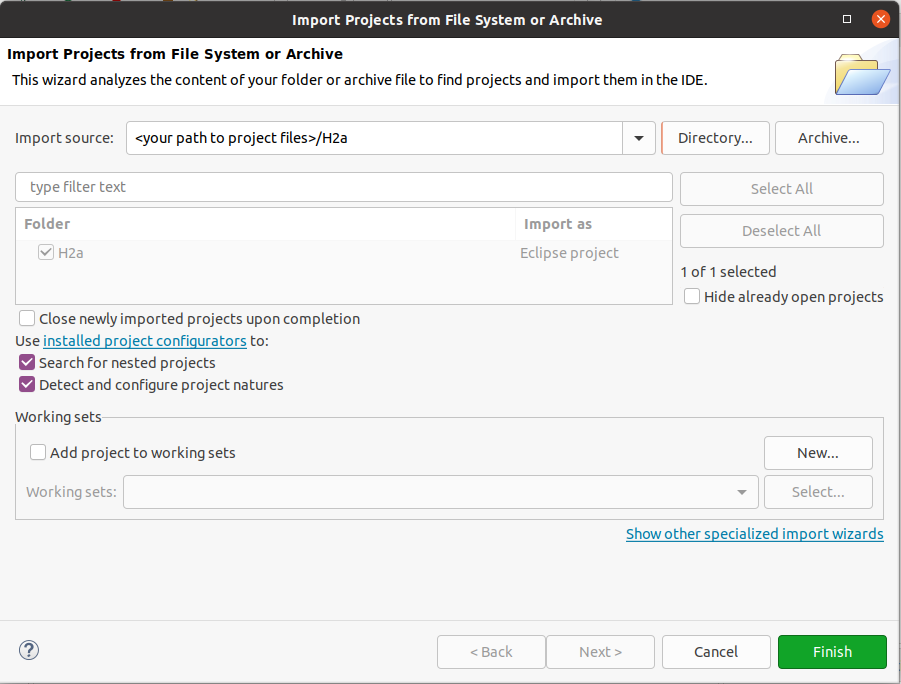
\includegraphics[scale=0.4]{figures/import_ide.png}
    \caption{IDE open project from file system window}
    \label{fig:import_ide}
\end{figure}
\begin{figure}[h]
    \centering
    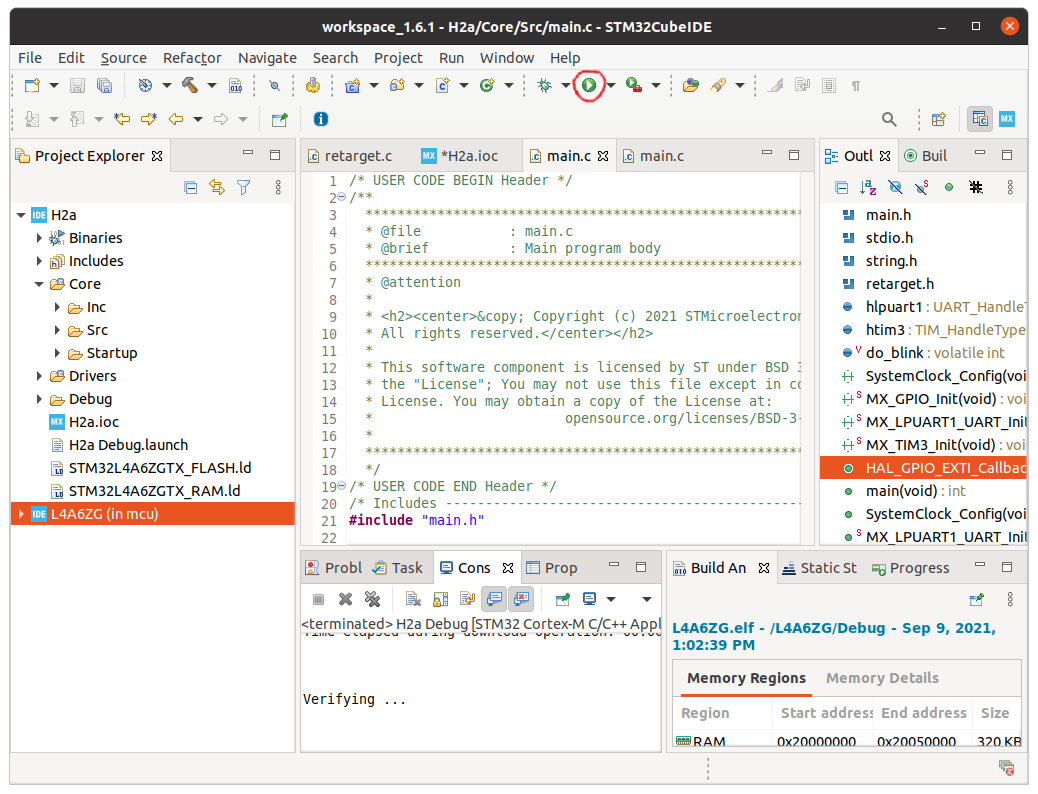
\includegraphics[scale=0.35]{figures/ide.png}
    \caption{STM32Cube IDE}
    \label{fig:cube_ide}
\end{figure}

You can now flash the MCU (i.e. program its Flash memory) with the baseline version of the code by using the USB cable. This is the first step that makes sure everything is working as expected. To do so, click on the button surrounded by the red circle in \autoref{fig:cube_ide}. The first time you launch a project, the IDE will prompt you the launch configuration. If you followed the tutorial correctly, the default options should fit your needs and you can directly click on \textbf{OK}. Consequently, the baseline version of the code should now be flashed on your MCU and it should be running properly: \textit{check that a green LED is blinking when you hold the blue button on the Nucleo MCU board}.

\begin{bclogo}[couleur = gray!20, arrondi = 0.2, logo=\bcinfo]{ST-Link programmer}
The ST-Link is a programmer and debugger. It provides the connection between your computer and the MCU on the board. It can be connected to your MCU with a connection called JTAG. In the case of the Nucleo MCU board, a dedicated ST-Link is soldered onto the board and is always connected to the MCU. It serves also as a USB to UART adapter.
\end{bclogo}

In order to read the messages that are sent from the MCU through the UART interface, you can open a terminal and write \texttt{screen /dev/ttyACM0 115200}\footnote{If it doesn't work, type \texttt{ls /dev | grep ttyACM}. If it gives you a result then use that instead of \texttt{ACM0}. Otherwise, the Nucleo MCU board is not connected to your computer or the USB passthrough for the VM is not properly configured.}, then press enter. Note that 115200 is the baudrate parameter. Now, you can see the messages coming from the UART. Press the black reset button to reset the MCU so that it sends "Hello World!" again. If you want to quit screen, you can use \textbf{Ctrl+a} to enter in command mode, then either type \textbf{$\backslash$}, \textbf{d} (to detach the screen) or \textbf{:quit}.
\begin{bclogo}[couleur = gray!20, arrondi = 0.2, logo=\bcinfo]{Serial communication baudrate }
The baudrate of a serial connection represents number of bits per second that are sent over the connection. This parameter must be identical between the transmitter (here the MCU) and the receiver (here the ST-link programmer on the Nucleo board that forwards the messages to your computer through USB). \end{bclogo}


\begin{bclogo}[couleur = gray!20, arrondi = 0.2, logo=\bcinfo]{Redirecting \texttt{stdout} to UART}
You can use the usual \texttt{printf} function family to print information via the UART stream. Note that this is not the case by default if you start a new project from scratch. For your information, the code that redirects \texttt{stdout} to the UART stream lies in \texttt{retarget.c}.
\end{bclogo}


\subsection{Using a state variable}

Have a look at the \texttt{main()} function and analyze its behavior. In particular, be sure that you understand the purpose of the HAL functions that are called.

\begin{bclogo}[couleur = gray!20, arrondi = 0.2, logo=\bcinfo]{Hardware Abstraction Layer (HAL)}
The MCU and its peripherals are controlled by memory-mapped registers. That is, in order to control them, one has to perform a read/write at a specific memory address (the address and value written determine the action performed -- you will find these in the reference manual of the MCU).
ST provides a HAL, which is a set of functions that abstract sequence of such reads and writes. We strongly recommend you to use it (see the HAL description document). Moreover, you need to know that there are two kind of HAL functions provided: the standard ones and the low level (LL) ones. The standard ones are easier to use than the LL ones. For this reason, we recommend you to stick to the standard HAL functions (without "\_LL\_").
\end{bclogo}

Let us now modify the LED behavior: we want the LED to toggle between blinking and no-blinking modes each time we press the button. Implement this using two boolean variables to store the current state of the system (button pressed or not, LED blinking or not). Then, flash the new version of your code and check that it is working as expected !

\begin{bclogo}[couleur = gray!20, arrondi = 0.2, logo=\bcattention]{STM32CubeIDE code generator}
Some of the code in \texttt{main.c} has been auto-generated by the IDE, and will be overwritten (soon) when we will change some configuration parameters.
When modifying your code, make sure to modify only the code that is between a USER CODE BEGIN and END (do not modify these comments). These parts of the code will not be overwritten, therefore preserving the changes you have implemented.
\begin{lstlisting}
  /* USER CODE BEGIN xxx */
     // insert your code here
  /* USER CODE END xxx */
\end{lstlisting}

If your project grows larger, you can also add your own \texttt{.c}/\texttt{.h} files (there is a menu for that). They are not overwritten by the code generator, except if there are collisions in the file names you and the code generator want to use. We therefore advise you to commit/backup your changes before running the code generator.
\end{bclogo}



%Analyze the behaviour of the MCU and identify at least one flaw of your implementation.


%\begin{bclogo}[couleur = gray!20, arrondi = 0.2, logo=\bcattention]{Debouncing a button}
%The button on the Nucleo is not perfect, when you press the button, it actually takes a small amount of time to stabilize the signal at the "pressed" state, and until then, it can switch back and forth. Taking this effect into account is called debouncing and it can be done either in hardware or in software. Let us try to do it in software. Basically, when a pressure on the button is detected, we must discard the subsequent pressures for a small amount of time. This can be naively done thanks to a delay function.
%\end{bclogo}

\subsection{Interrupt-based programming}

As your code is implemented using a polling strategy (i.e., the state of the system is regularly checked, and appropriate action is taken). This approach has several drawbacks, one of them being the complexity to handle multiple tasks at the same time. For instance, if you quickly press the button when your code is executing a delay with the \texttt{HAL\_Delay()} function, the button press can not be detected. While this limitation can be fixed, polling multiple peripherals and running multiple time-delayed actions in parallel will quickly make your code very complex and most likely less robust to unexpected behaviors.

You will now switch your software to an interrupt-based implementation. As seen in the L2 lecture, the interrupt stops the main activity of the processor and switches to the action to be done when a specific event is detected. In our case, we will set up the MCU such that on a rising edge on the button GPIO, the MCU enters in a function where we can set the blinking state of our system.

\begin{bclogo}[couleur = gray!20, arrondi = 0.2, logo=\bcinfo]{Interrupts terminology}
An interrupt originates from an interrupt request (IRQ) which can originate from outside the MCU (typically an event on a GPIO pin), from an MCU peripheral (e.g. a timer) or from the software (by writing to a specific register). The IRQ is handled by the interrupt controller (a hardware component of the MCU), which then runs the interrupt handler, also named interrupt service routine (ISR), or callback (this is the name used by the ST HAL).
\end{bclogo}

To do so, we first need to set the GPIO pin linked to the button in interrupt mode. The IDE provides an easy way to this, in your source files, open the file \textbf{\texttt{H2a.ioc}}. It is a configuration file for all the parameters of the MCU, peripherals, clock tree and project. If it is not your case by default, open the \textbf{Pinout \& Configuration} tab. On the left of the screen, you see all the available peripherals on the MCU. You can click on a peripheral to open a panel where you can set its parameters. In the main panel, you see the different pins of the MCU and their modes. Here, you can click on each pin and set its functionality.

Find the pin PC13 connected to the blue button. You can observe that it is set as GPIO input. To be able to trigger interrupts, we need to use the GPIO EXTernal Interrupt mode: \texttt{GPIO\_EXTI}. Select it when clicking on the pin as illustrated in \autoref{fig:gpio_exti_select}. Note that the name of the pin changed. Change it back to B1 by right-clicking on the pin. Now, we need to set up the parameters of Nested Vector Interrupt Controller (NVIC) such that it processes the signal sent by the GPIO pin. To do so, click on NVIC under System Core in the left panel. You will see a panel appear as in \autoref{fig:nvic_params}. Here you can select which interrupts you want to enable or not. Some of the interrupts cannot be disabled. You need to activate here the EXTI line. That's all we need to do in the parameters. You can save the \texttt{.ioc} file, the IDE will prompt you to regenerate the code based on your modifications, answer yes (remember: that is the reason why you need to write your custom code in the USER CODE areas!).

\begin{bclogo}[couleur = gray!20, arrondi = 0.2, logo=\bcinfo]{GPIO Interrupt trigger parameters}
By default, the MCU is configured such that a rising edge of the GPIO pin triggers an interrupt request (IRQ) to the CPU. This corresponds to pressing the button (checkout the schematic of the MCU board to understand why!). It is possible to configure it for alternate events, such as a falling edge, corresponding to the release of the button. To do so, open the parameters of the GPIO peripheral under System core in the \texttt{.ioc} file, select the GPIO tab in the parameter panel and select the pin that you want to configure. You can change the edge detection in the GPIO mode setting in the lower part of the screen.
\end{bclogo}

When an IRQ is triggered, the NVIC makes the CPU call and interrupt handler function. With the ST HAL, you can write code to be executed in the handler in a ``callback'' function. In your main file, insert the EXTI interrupt callback function as below.

\begin{lstlisting}[columns=fullflexible]
void HAL_GPIO_EXTI_Callback(uint16_t GPIO_Pin) {
    if (GPIO_Pin == B1_Pin) {
        // Insert code to be executed in the interrupt
    }
}
\end{lstlisting}
This function will be called each time a GPIO EXTI interrupt is raised, whatever the concerned pin. This is why we need the if condition to check which pin was triggered. Now, remove the GPIO read function from your main loop and update your state variable in the callback function of the interrupt handler.

\begin{bclogo}[couleur = gray!20, arrondi = 0.2, logo=\bcattention]{Data races and volatile variables in C}
Your state variable will be a global variable, such that it can be modified in the main function and in the interrupt handler.
The main function and the interrupt handler are concurrent: they are not part of the same ``execution flow'', similarly to threads that run under an OS.
With all concurrent programming, you have to be careful the access to variables that are shared (i.e., read or written from more than one execution flow).
If at least one of the execution flow writes to a variable (concurrent reads are always ok!), the result of the execution might be non-deterministic (e.g., depend on the exact way the execution flows are interleaved), which is called a data race.
For instance, if you increment a variable (which makes 3 instructions: load, add and store) both from \texttt{main()} and from an interrupt handler, you have a data race if you take no extra precaution: if the \texttt{main()} is interrupted just after the load, the variable gets incremented by only 1 instead of 2.
In order to avoid data races, all concurrent read and writes should be either atomic (roughly, a single load/store) or synchronized (through locks, etc.).

This is further complicated by the semantics of the C programming language: it is such that the compiler can (almost) assume that there is no concurrent execution.
Therefore, if a program does not read a variable from the \texttt{main()} execution flow, it may ``optimize'' your \texttt{main()} by discarding writes to this variable, as they are ``useless''.

As a result, whenever a variable is \textbf{shared} (i.e., accessed by multiple execution flows), or represents a \textbf{memory-mapped control register}, you have to make it \textbf{volatile}. This is done by putting the qualifier \texttt{volatile} before the type in the declaration of the variable.

\textit{This was only a very limited introduction! To go further: \url{https://blog.regehr.org/archives/28}. You may also search the keywords: C memory model; atomic memory access ordering; memory barrier.}
\end{bclogo}

\begin{bclogo}[couleur = gray!20, arrondi = 0.2, logo=\bcinfo]{Interrupt callback good practice}
Be careful not to lock-up your processor: if you have a long-running interrupt handler, the MCU might not be able to respond to other events that happen.
The two common solutions are to delegate the long processing to the \texttt{main()} (and communicate that the processing should be performed by setting a state variable in the interrupt handler), or to configure the priority of the long-running interrupt such that it can be interrupted by other, higher priority, interrupts. Be careful as usually, the highest priority has the lowest value i.e. 0 being the highest priority as shown in \autoref{fig:nvic_params}.
\end{bclogo}

\begin{figure}[h]
    \centering
    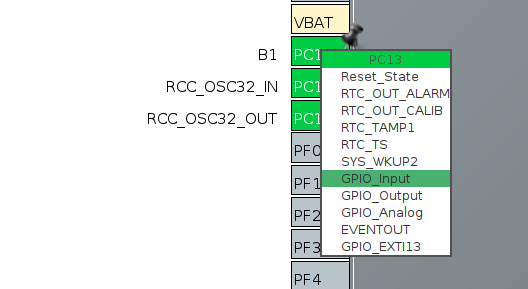
\includegraphics[scale=0.4]{figures/gpio_exti_select.png}
    \caption{Cube MX GPIO pin mode selection}
    \label{fig:gpio_exti_select}
\end{figure}

\begin{figure}[h]
    \centering
    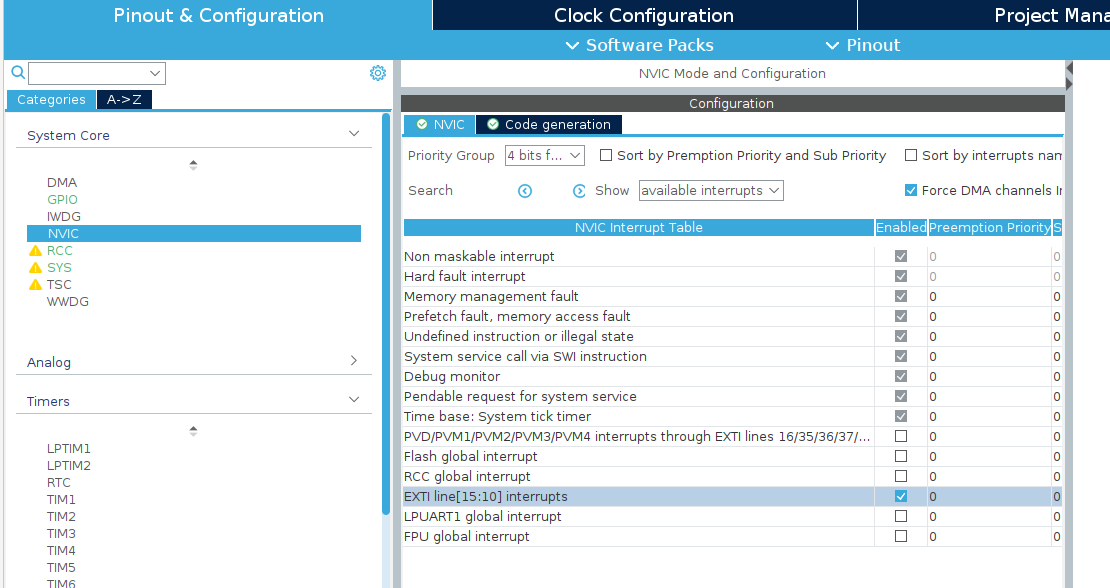
\includegraphics[scale=0.4]{figures/nvic_exti_select.png}
    \caption{NVIC parameter selection}
    \label{fig:nvic_params}
\end{figure}


\subsection{Using a TIMER to blink a LED}
Now that you have a code that uses interrupts to detect a press on the button, you will use a more advanced way to blink the LED. Imagine your MCU has to blink its LED at a very specific frequency and must at the same time, perform heavy calculations. In such cases, the blinking might be altered due to the computation time of the other task of the MCU. This can be avoided by using a peripheral of the MCU to move the task of blinking from the MCU to this peripheral called \textbf{timer}.

Timers are simple circuits that increment a register by 1 at each clock cycle and perform additional actions when certain conditions are met. Such actions can be reading or writing to a GPIO pin, triggering interrupts and more. A typical condition for a timer is \textbf{comparing} the value of the counter to an other (fixed) value, and triggering an action whenever the two values are equal.

We will now show you how to setup the timer. A timer has multiple channels that can each perform a condition-action pair. Each channel can be linked to at most one of the few GPIO pins that it is connected to. On the device you have for the project, there are several timers available. For determining which timer channels are linked to which GPIO pins, you can take a look at the datasheet of the MCU. In our case, the blue LED is connected to PB7, which can be connected the channel 2 of timer 4. To do so, open the \texttt{.ioc} file and the \textbf{Pinout \& configuration} tab and look for pin PB7. When clicking on it, choose \textbf{TIM4\_CH2} as in \autoref{fig:tim_pc7}.
\begin{figure}[h]
    \centering
    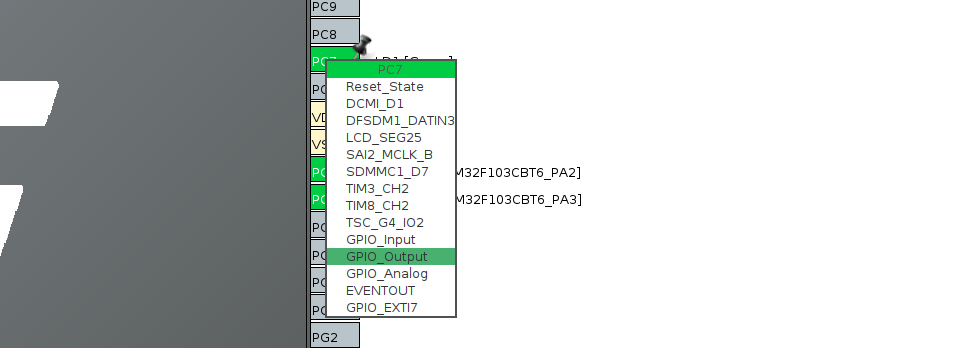
\includegraphics[scale=0.4]{figures/timer_pc7.png}
    \caption{Possible uses for pin PC7}
    \label{fig:tim_pc7}
\end{figure}
Still in the \texttt{.ioc} file, we will now enable the timer \textbf{TIM4}. Click on the name of this peripheral in the leftmost column of the \texttt{.ioc} window, in the submenu \textbf{Timers}. You should see all the parameters of TIM4 in a new panel. In the \textbf{mode} panel, you should set the clock source to \textbf{Internal clock} and channel 2 to \textbf{Output compare CH2}, the rest should remain disabled. In the configuration panel, you should set the \textbf{Prescaler, Counter Mode, Counter Period and Mode} as in \autoref{fig:tim_settings}.

\begin{figure}[h]
    \centering
    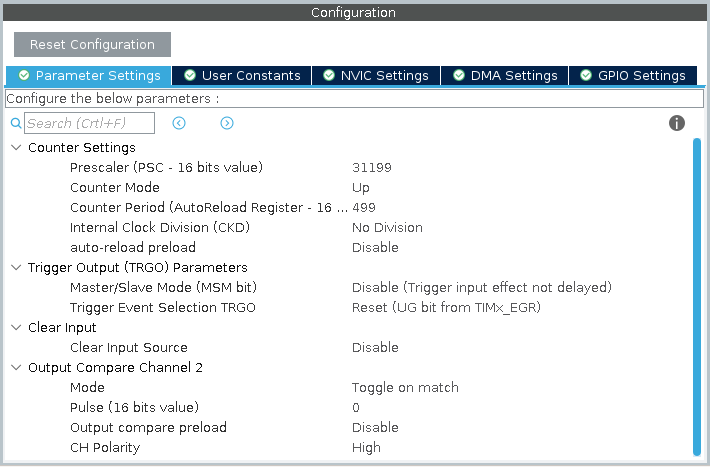
\includegraphics[scale=0.65]{figures/tim_settings}
    \caption{Timer settings}
    \label{fig:tim_settings}
\end{figure}


\begin{bclogo}[couleur = gray!20, arrondi = 0.2, logo=\bcquestion]{Timer parameters analysis}
\begin{itemize}
    \item Take a look at the mode and the proposed values. Try to calculate the frequency of the blinking without launching the code. (Hint: start by checking what is the clock frequency feeding your timer peripheral in the \textbf{Clock Configuration} panel of the \texttt{.ioc}).
    \item Now, change the Pulse value to anything between 0 and the counter period and describe what happens.
    \item What happens when you set a pulse value above the counter period?
\end{itemize}
\end{bclogo}

\begin{bclogo}[couleur = gray!20, arrondi = 0.2, logo=\bcinfo]{Timer parameters detailed}
\begin{itemize}
    \item Take as example an MCU clock that runs at 8MHz the timer triggers an event every second, this means that a 16-bit timer is not suitable as the compare register should be set at 8000000, but it's maximal value is 65535. This is why we have \textbf{prescalers}, which make the timer counter register increment every \texttt{prescaler value} cycles. Therefore, the update frequency $f_{update}$ is given by $f_{update} [Hz] = \frac{TIM\_CLK}{(PSC+1)(PRD+1)}$, where $PSC$ is the prescaler value and $PRD$ the period value.
    \item The counter period is the maximal value of the counter, i.e. at the next cycle, the counter value will reset to 0.
    \item The pulse parameter contains the value to compare to the timer counter.
    \item Mode contains the action to perform on channel 2.
 \end{itemize}
\end{bclogo}


Now that you have everything set up in the \texttt{.ioc} file, you can regenerate your code by saving the \texttt{.ioc}. The two functions that you will need to use the timer are:
\begin{itemize}
    \item \texttt{HAL\_TIM\_OC\_Start(\&htim4, TIM\_CHANNEL\_2);} to start the timer and the blinking.
    \item \texttt{HAL\_TIM\_OC\_Stop(\&htim4, TIM\_CHANNEL\_2);} to stop the timer and the blinking.
\end{itemize}
You can now write a simple code that takes advantage of both the interrupt for the button and the timer. Therefore, your new code (not the one generated by CubeMX) should not contain any call to \texttt{HAL\_GPIO\_...} functions, as the LED pin is not in GPIO mode anymore.

\begin{bclogo}[couleur = gray!20, arrondi = 0.2, logo=\bcattention]{\texttt{main} infinite loop}
In bare-metal embedded programming, the \texttt{main} function must never return, otherwise the processor might to execute random pieces of memory. Therefore, the \texttt{main} must always contain an infinite loop. This loop may be as simple as \texttt{while (1) \{\}}, if there is nothing to do.
\end{bclogo}

\vspace{-0.3cm}
\subsection{Introduction to power consumption monitoring}
Now that you don't have any code left in the main loop, what can we do with it? As we are developing an embedded solution, we have an energy budget determined by the capacity of a battery or by the energy that we can harvest from the environment (or both of them). Therefore, we want to find a solution which has the lowest power consumption to extend the lifetime of our device and/or having our solution functional most of the time.

An easy way to measure instantaneous power consumption is using an ammeter. You simply need to break the power supply line of the MCU and insert the ammeter. Hopefully, this is made easy with a removable jumper placed on the Nucleo MCU board. Find the jumper \textbf{JP5} on the Nucleo MCU board, which is located near the LED that is used for blinking as shown in \autoref{fig:JP5}. Remove the jumper and \textbf{DO NOT LOSE IT}! Set up the multimeter in ammeter mode in the mA range and observe the values.

\begin{figure}[h]
    \centering
    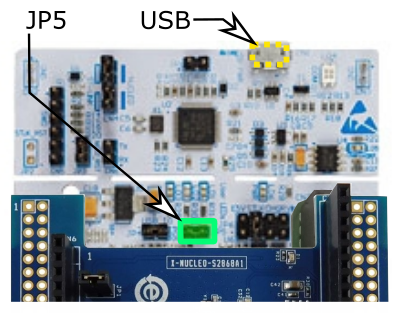
\includegraphics[scale=0.5]{figures/JP5}
    \caption{Remove JP5 to be able to measure the current drawn by the MCU.}
    \label{fig:JP5}
\end{figure}

\begin{bclogo}[couleur = gray!20, arrondi = 0.2, logo=\bcinfo]{Good practice regarding measurement instruments}
It is always a good practice to test your measurement instruments on a reference signal before starting measuring what you need. It might sounds obvious, but in practice it can happen that your probe or cable is broken, a blown fuse, ... \end{bclogo}

An other method to measure the current of the MCU is using a series resistor called shunt resistor as in \autoref{fig:measure}. You need to probe the two sides of the resistor to calculate its voltage drop and then apply Ohm's law to find the current. When measuring with an oscilloscope, the sampling rate of the scope is much faster than the one of the multimeter, therefore it is better to use this method in case of rapid, high consumption current peaks, such as a wireless packet transfer. Practically, you can replace the jumper by a resistor of your chosen value on the pins of \textbf{JP5}. You can \textbf{NOT} probe the voltage drop with one probe because the ground pin can \textbf{MUST} be connected to ground.
\begin{figure}[h]
    \centering
    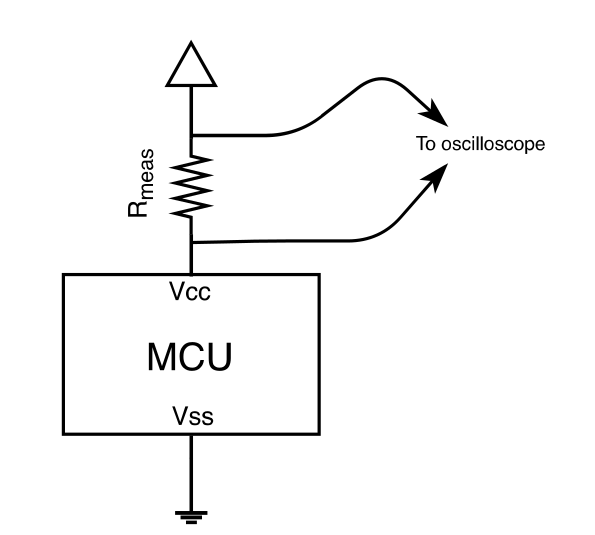
\includegraphics[scale=0.3]{figures/measuring.png}
    \caption{How to measure the current of an MCU.}
    \label{fig:measure}
\end{figure}

\begin{bclogo}[couleur = gray!20, arrondi = 0.2, logo=\bcattention]{Choosing the right shunt resistor value}
The resistor that you choose has a huge impact on your measurements, having a too small voltage drop compared to the noise floor of your oscilloscope will lead to wrong measurements, but having a too high voltage drop will lead to a Brown-Out-Reset, where the MCU resets itself because there is not enough voltage. In the case of the STM, the minimal VDD is 1.71V.\end{bclogo}

\begin{bclogo}[couleur = gray!20, arrondi = 0.2, logo=\bcquestion]{Comparing empty while loops}
We want you to compare the power consumption of 3 different ways of doing nothing in the main loop:
\begin{itemize}
    \item The first one is already implemented in your code, it is having an empty \texttt{while(1)} loop.
    \item Now, add a \texttt{HAL\_Delay} function in the loop of arbitrary delay.
    \item Instead of the delay function, put the MCU to sleep mode by calling \texttt{\textbf{\_\_WFI()}} which stands for \textit{wait for interrupt}.
\end{itemize}

This is just a really basic introduction to the power modes management: the goal here is to realize the strong link between your code and the power consumption of your solution. Later in the project, you will learn more about these considerations and implement mode advanced power saving modes.

\end{bclogo}
\subsection{(OPTIONAL) To go further: Debugging your code}

If you already got involved in some kind of programming, you know that it never goes as expected at the first shot (at least, not often). You therefore need to start debugging your code to understand where things go wrong and fix the issue. Of course, you can use \texttt{printf}'s to debug your code. However, as it has been said before, the ST-Link is also a debugger. We can halt the MCU at a specific line of code, look at the values of variables and registers, advance in the code step by step, and many others functionalities. To access the debugger mode, you need to launch your code with the "green bug" button just on the left of run button you use for normal flashing. You can switch to the debugger perspective as proposed by the IDE.
Next, we detail how to use the debugger functionalities :
\begin{itemize}
    \item \textbf{Breakpoints} : are lines or code that trigger a halt on the MCU. They allow to stop the MCU at a specific line of code, and observe its state. To set up a breakpoint, simply double click on the line number where you want to put your breakpoint. The MCU will halt before the execution of this line. You should see a small blue point at the left of the line number as in line 93 of \autoref{fig:breakpoint}

    \begin{figure}[h]
    \centering
    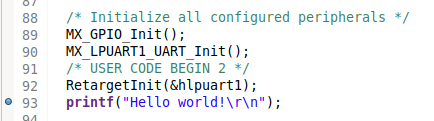
\includegraphics[scale=0.6]{figures/breakpoint.png}
    \caption{Breakpoints in the IDE}
    \label{fig:breakpoint}
    \end{figure}

    \item \textbf{Step by step execution} : of the code is performed thanks to the buttons in the toolbar as in \autoref{fig:debugtools}. The play and pause buttons allow starting and stopping the MCU, and the 3 rightmost buttons allow advancing step by step in the code.

    \begin{figure}[h]
    \centering
    
\includegraphics[scale=0.6]{figures/debugging.png}
    \caption{Debugging toolbar}
    \label{fig:debugtools}
    \end{figure}

    \item \textbf{Register values } : can be observed in the right panel. The \textbf{register} tab contains the values of the registers of the ARM Cortex and the \textbf{SFR} (Special Function Register) tab as shown in \autoref{fig:sfr_values} contains the values of the peripheral registers.

    \begin{figure}[h]
    \centering
    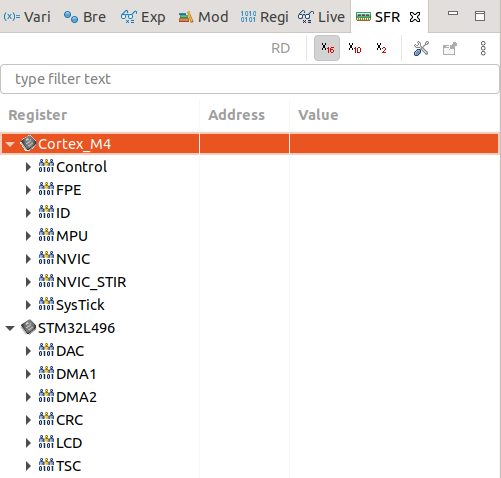
\includegraphics[scale=0.3]{figures/debug_peripherals.png}
    \caption{Special function register values}
    \label{fig:sfr_values}
    \end{figure}

\end{itemize}

\newpage
\begin{bclogo}[couleur = gray!20, arrondi = 0.2, logo=\bcquestion]{Getting used to the debugger}
\begin{itemize}
    \item Set up a breakpoint at the line of the "Hello World!" \texttt{printf}. Launch the debugger and observe that it does not print anything in the serial console.
    \item Now, advance step by step with your code until you reach the line where you start your timer. Take a look at the registers of TIM3 and observe the changes. (You can compare what you observed with the reference manual of the MCU.)
\end{itemize}
\end{bclogo}

Finally, when you debug real-time software, don't forget that, when reaching a breakpoint, your code is not real-time anymore ! A few \texttt{printf} can also be helpful\dots

\begin{bclogo}[couleur = gray!20, arrondi = 0.2, logo=\bcattention]{Don't abuse of \texttt{printf}s}
Be aware that the \texttt{printf} function is hungry in CPU cycles. If you decide to print too much information and use a slower clock speed on your MCU, you might miss real-time constraints.
\end{bclogo}

\section{Demo D5: double buffering acquisition and classification}
%
During this LELEC2102 project, we expect you to be able to present quick demos on specific topics, as scheduled in the program for this semester. They can be seen as small checkpoints to make sure you master the important basic blocks of the project. These demos should take you less time than writing a detailed report while still providing a good occasion to develop new skills, learn by doing and finally get some feedback along the way! There is no need to write anything for a demo but you must make sure it will run "live" smoothly. \\
\\
The \textbf{demo D5 on Friday December 1$^{\text{st}}$ 4.15 PM} will consist in checking you master the provided code and you will be able to modify it accordingly for some improvements during the second semester. For this demo on Friday, we expect you to:
%
\begin{itemize}
    \item Show an acquisition of a full feature vector from a single button press.
    \item Show a feature vector-long melspectrogram acquired with the jack cable, then with the microphone.
    \item Show a classification result obtained live from acquisition with your MCU.
\end{itemize}



\end{document}

%%%%%%%%%%%%%%%%%%%%%%%%%%%%%%%%%%%%%%%%%%%%%%%%%%%%%%%%%%%%%%%%%%%%%%%%%%%%
